%% INISTA 2026 submission — mlcompass evidence-bound runtime schema
%% IEEE conference template (IEEEtran). Compiles with pdflatex on Overleaf
%% out of the box: the bibliography is embedded (no bibtex step required).
\documentclass[conference]{IEEEtran}
\IEEEoverridecommandlockouts

\usepackage[utf8]{inputenc}
\usepackage[T1]{fontenc}
\usepackage{cite}
\usepackage{amsmath,amssymb,amsfonts}
\usepackage{graphicx}
\usepackage{booktabs}
\usepackage{textcomp}
\usepackage{url}
\usepackage{xcolor}

\begin{document}

\title{An Evidence-Bound Runtime Schema for Reliable LLM Narration\\of Machine-Learning Pipeline Evidence}

\author{%
\IEEEauthorblockN{Hakan Sabuni\c{s}\IEEEauthorrefmark{1},
Yusuf \"Unl\"u\IEEEauthorrefmark{1},
Selim Aky\"oku\c{s}\IEEEauthorrefmark{2}}
\IEEEauthorblockA{Department of Computer Engineering, Istanbul Medipol University, Istanbul, T\"urkiye\\
\IEEEauthorrefmark{1}Student \quad \IEEEauthorrefmark{2}Advisor\\
\{hakan.sabunis, yusuf.unlu\}@std.medipol.edu.tr, \quad sakyokus@medipol.edu.tr}%
}

\maketitle

\begin{abstract}
Large language model (LLM) agents are increasingly placed as an advisory layer over deterministic software tools: the agent invokes a tool, receives structured output, and narrates it in natural language for a human operator. We address a specific reliability failure of this pattern, \emph{phantom-entity fabrication}, in which the narrator cites entities---column names, defects, or fixes---that are absent from the upstream deterministic evidence. In a machine-learning (ML) engineering setting this failure is actively harmful: a confidently fabricated diagnosis is worse than silence, because the operator trusts the tool and chases a nonexistent cause. Mainstream constrained-generation and schema-validated tool-use mechanisms enforce constraints that are \emph{declared statically} at authoring time; we instead make the constraint data-dependent. We present an \emph{evidence-bound runtime schema} in two tiers: (i)~the \texttt{enum} domain of the narrator's tool-input field is generated from the deterministic evidence dictionary at call time, and (ii)~the returned citations are deterministically re-validated against that evidence set, rejecting-and-retrying on a violation and stripping any residual out-of-evidence entity. Tier~(ii) gives a \emph{provider-independent} worst-case guarantee: every response that passes the contract cites only entities present in the evidence, by construction. We instantiate the contract in \textbf{mlcompass}, an open-source ML-pipeline assistant, where it ships in the narrator that investigates suspiciously perfect metrics (a classic symptom of data leakage). On a controlled synthetic regression task, measured live against a commercial LLM endpoint, the \emph{observed} user-facing fabrication rate falls from 56.5\% (bare prompt) to 0.0\% (strict prompt) to 0.0\% (evidence-bound contract) over $N=200$ responses per configuration, with Wilson 95\% confidence intervals reported. We frame the result honestly: on this model the strict prompt alone eliminated every observed violation, so the contract's contribution is not a lower observed rate but the structural guarantee on the residual tail (Wilson upper bound 1.88\% at 0/200) --- a guarantee that holds even where prompt efficacy regresses.
\end{abstract}

\begin{IEEEkeywords}
Agentic AI, large language models, hallucination mitigation, constrained generation, tool use, data leakage, machine-learning tooling.
\end{IEEEkeywords}

\section{Introduction}
Modern machine-learning engineering is supported by a fragmented ecosystem of single-purpose tools: profiling libraries for dataset inspection~\cite{ydata}, experiment trackers for training~\cite{mlflow,tensorflow}, automated model search for selection~\cite{autosklearn}, and container tooling for deployment. Each covers one slice of the pipeline; none gives end-to-end advice, and none carries state across stages. A natural response is to place a large language model (LLM) on top as an advisory layer---an \emph{agent} that calls these tools, reads their structured output, and explains it to the engineer. This is the agentic pattern formalized by ReAct~\cite{react} and Toolformer~\cite{toolformer} and operationalized by tool-integration standards~\cite{mcp}.

The pattern has a well-documented hazard: LLMs hallucinate~\cite{ji,huang}. General-purpose code assistants built on the same foundation models~\cite{codex} still fail on real software tasks at substantial rates~\cite{swebench}. In an advisory ML setting the danger is specific and acute. When the narrated object is \emph{structured evidence}---a dictionary of measured facts produced by a deterministic tool---the agent can introduce what we call \textbf{phantom-entity fabrication}: it names a column, a defect, or a remedy that is \emph{not present} in that evidence. This is a closed-world \emph{extrinsic} faithfulness failure in the taxonomy of Ji \emph{et al.}~\cite{ji}: the cited entity has no support in a source that is fully enumerable. A fabricated diagnosis delivered with fluent confidence is worse than no diagnosis at all, because the practitioner acts on it.

A reasonable mitigation is \emph{constrained generation}: restrict the model's output to a formal structure. Outlines~\cite{outlines}, LMQL~\cite{lmql}, grammar-constrained decoding~\cite{gcd}, and Guidance~\cite{guidance} enforce a grammar or schema during decoding, and every major provider now validates tool-call inputs against a declared JSON schema~\cite{structured}. These mechanisms can already be driven by \emph{input-dependent} grammars~\cite{gcd} and per-request schemas; the capability to vary a schema with the input exists. What is missing is the \emph{discipline of binding the value domain to the deterministic evidence and verifying it independently}. A schema declared at authoring time guarantees that a field named \texttt{columns\_referenced} holds \emph{a string}; unless the author actively rebuilds it, it does not know that, for \emph{this dataset at this call}, the only legitimate strings are a specific small set. And even a per-call schema offers no guarantee unless the provider's enforcement is trusted---which, for a safety claim, it should not be.

We close this gap with an \textbf{evidence-bound runtime schema} in two tiers. \emph{Tier~A (constrained generation):} the \texttt{enum} domain of the narrator's tool-input field is generated \emph{at call time} from the deterministic evidence dictionary, so the permitted entities are exactly the set the upstream layer observed. \emph{Tier~B (deterministic validation):} the returned citations are re-checked against that evidence set in pure Python; a violation triggers a corrective retry, and any residual out-of-evidence entity is stripped before the response reaches the user. Tier~B makes the guarantee real: \emph{every response that passes the contract cites only entities present in the evidence, by construction, independent of the provider}. We are explicit that Tier~B alone is, in essence, a membership check over the evidence keys; the contribution is not that check but (a)~framing phantom-entity fabrication as a decidable closed-world faithfulness failure, (b)~binding the constrained-generation domain to runtime evidence so the model is biased away from violations in the first place, and (c)~combining the two into a provider-independent guarantee that we measure.

We instantiate the contract in \textbf{mlcompass}, an open-source (MIT) ML-pipeline assistant. The narrator we study ships in production and is triggered automatically when a deterministic metric looks impossibly good (e.g., $R^2 > 0.999$)---the canonical signature of data leakage~\cite{leakage}, a high-stakes, easily-missed error.

The paper makes three contributions:
\begin{enumerate}
\item We articulate \emph{phantom-entity fabrication} as a distinct, decidable reliability failure of LLM agents that narrate structured evidence, and identify why statically-declared constrained generation does not prevent it (Sec.~\ref{sec:related}, \ref{sec:contract}).
\item We propose the two-tier \emph{evidence-bound runtime schema} and measure its effect in a live three-configuration ablation ($N=200$, Wilson 95\% CIs): the observed user-facing fabrication rate drops from 56.5\% under a bare narrator to 0.0\% under both the strict prompt and the full contract --- which is exactly why we lead with the structural guarantee rather than the point estimate (Sec.~\ref{sec:experiments}).
\item We report engineering findings from deploying the contract inside a real multi-surface tool, including a cross-surface state-parity hazard (Sec.~\ref{sec:parity}, \ref{sec:disc-parity}).
\end{enumerate}

\section{Related Work}
\label{sec:related}
\textbf{Hallucination and faithfulness.} Ji \emph{et al.}~\cite{ji} survey hallucination across generation tasks and distinguish intrinsic (contradicting the source) from extrinsic (unverifiable from the source) failures; Huang \emph{et al.}~\cite{huang} give an LLM-specific taxonomy. Phantom-entity fabrication is an extrinsic failure with a special structure: the ``source'' is a finite, machine-enumerable evidence dictionary, which makes the faithfulness check \emph{decidable} rather than open-world. Our work eliminates one decidable slice of it at the tool boundary.

\textbf{LLM agents and tool use.} ReAct~\cite{react} interleaves reasoning with tool actions, and Toolformer~\cite{toolformer} shows models can learn when and how to call external APIs. Tool-integration standards~\cite{mcp} let LLM clients discover and call third-party tools over a uniform protocol. These establish \emph{how} agents act; they do not constrain \emph{what} an agent may say about a tool's output. Our contract sits at that under-specified boundary.

\textbf{Constrained and structured generation---the closest prior art.} Outlines~\cite{outlines} reformulates guided decoding as transitions over a finite-state machine. LMQL~\cite{lmql} adds declarative constraints over a typed grammar. Grammar-constrained decoding~\cite{gcd} guarantees grammatical validity without fine-tuning and \emph{explicitly supports input-dependent grammars}. Guidance~\cite{guidance} enforces JSON-schema and regex constraints at the token level, and provider tool-use APIs validate calls against a declared JSON schema~\cite{structured}. We do not claim that varying a constraint with the input is new---\cite{gcd} already does. Two things distinguish our setup. First, we bind the value domain specifically to a \emph{deterministic evidence producer}, so the constraint tracks ground-truth observations rather than task structure. Second, we do not rely on the decoder or provider to enforce it: a deterministic post-validation makes the guarantee hold even if the provider admits an out-of-enum token. The combination---evidence-bound domain plus provider-independent verification, framed around a decidable faithfulness failure---is, to our knowledge, not described as a contract in this literature.

\textbf{Code assistants and their reliability.} Foundation models trained on code~\cite{codex} power widely-used assistants, yet they resolve only a fraction of real-world software issues~\cite{swebench} and, in our informal pre-project trials, silently accepted training scripts with semantically invalid configurations (e.g., a \texttt{momentum} argument to an optimizer that does not accept one). General-purpose assistants target syntactic correctness; ML-pipeline tooling must target domain-specific semantic correctness---without fabricating.

\textbf{ML pipeline tooling.} Profiling libraries~\cite{ydata} produce descriptive statistics but have no notion of a target column. Experiment trackers~\cite{mlflow,tensorflow} record per-run metrics without interpreting plateaus or overfitting. Automated model search~\cite{autosklearn} selects estimators without narrating \emph{why}. mlcompass adds a state-carrying advisory layer over the same artifacts; the contribution of \emph{this paper} is the reliability contract that makes its narrator safe, not the tool surface.

\section{Methodology}
\subsection{Threat Model}
We assume an honest operator and a well-behaved LLM provider---no adversarial weight poisoning, no malicious operator. The risk we address is the model's tendency to fabricate entities under output-distribution pressure on edge-case inputs. We explicitly do \emph{not} address: (i)~adversarial column names in user data attempting prompt injection; (ii)~provider outages or fabricated \emph{content about} a correctly-cited evidence item; or (iii)~miscalibrated confidence on a correctly-cited item. These residual risks are discussed in Sec.~\ref{sec:limits}.

\subsection{System Architecture}
mlcompass is organized into three layers (Fig.~\ref{fig:arch}). \emph{Surfaces:} eleven pipeline tools are exposed through a CLI, a tool-integration server~\cite{mcp} for compatible LLM clients, an autonomous agent, and slash commands for coding assistants---all routing to one deterministic backend. \emph{Two-layer brain:} the deterministic evidence layer is pure Python and always returns a structured dictionary (never free text), so every command has a fully offline path; the optional LLM narrator receives that dictionary and explains it, running only when requested. \emph{Persistent context:} a \texttt{.mlcompass/} folder persists project metadata, a chronological decision log, and dataset/run records across invocations.

\begin{figure}[t]
\centering
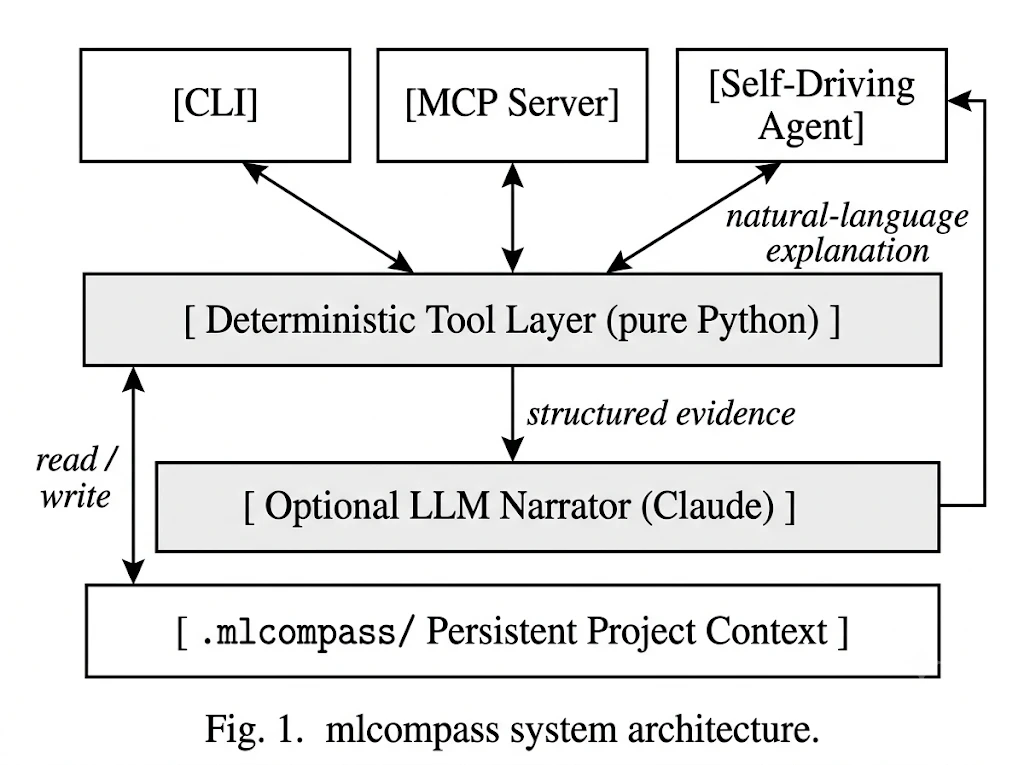
\includegraphics[width=\columnwidth]{architecture.png}
\caption{System architecture. Four surfaces sit on a two-layer brain---a deterministic tool layer plus an optional LLM narrator---over a persistent project-context folder. The evidence-bound schema is generated at the tool-to-narrator boundary, and the narrator's citations are re-validated against the evidence before they reach the user.}
\label{fig:arch}
\end{figure}

\subsection{The Evidence-Bound Contract}
\label{sec:contract}
We describe the contract through the automatic leakage investigation~\cite{leakage} triggered when an evaluation observes a suspicious metric ($\mathrm{AUC} > 0.995$, accuracy $> 0.99$, or $R^2 > 0.999$).

\textbf{Layer~1 --- Deterministic evidence producer.} A pure-Python module reads the predictions table and emits a structured dictionary $E$ containing (i)~the suspicious metric; (ii)~per-feature correlations against the target $y$, reported as $\max(|\rho_P|,|\rho_S|)$ with $\rho_P$ and $\rho_S$ the Pearson and Spearman correlations; (iii)~a candidate-leak set $C = \{\, c : \max(|\rho_P(c,y)|,|\rho_S(c,y)|) \geq 0.99 \,\}$; and (iv)~the perfect-match rate $P(\hat{y}=y)$. Spearman is reported alongside Pearson because monotone target transforms ($\log y$, $\sqrt{y}$, $\alpha y + \beta$) weaken $\rho_P$ while leaving $\rho_S = 1.0$; without it, a log-target leak at $\rho_P \approx 0.94$ would slip past a Pearson-only filter.

\textbf{Layer~2 --- Strict-prompted narrator.} The narrator receives $E$ with a system prompt: cite only items present in $E$; emit \texttt{cannot\_determine} rather than guess; downgrade confidence on small samples; and propose only manual checks, never code patches.

\textbf{Layer~3 --- Evidence-bound runtime schema (two tiers).} The narrator answers through a \texttt{submit\_investigation} tool, and the contract enforces evidence-faithfulness in two tiers.

\emph{Tier~A --- runtime enum.} The tool's \texttt{columns\_referenced} field is restricted by a JSON-schema \texttt{enum} \emph{generated at call time} from $E$: the domain is $C \cup \{\text{features reported in the correlation pass}\}$, i.e., exactly the columns the deterministic layer observed. This biases the decoder toward valid citations and is the constrained-generation half of the contract.

\emph{Tier~B --- deterministic validation.} When the tool input returns, every cited column is re-checked against the evidence set in pure Python---\emph{not} trusting the provider's enum enforcement. On a violation the contract issues a corrective retry (naming the offending column and the permitted set), up to two attempts; any column still outside the evidence set after the retry budget is removed before the response reaches the user. Tier~B yields the worst-case invariant: \emph{for any response the contract returns, every cited column $\in E$, by construction.} We are explicit that this final check is, in isolation, a set-membership filter over $E$'s keys; its value is that it makes the guarantee provider-independent and offline-testable, while Tier~A reduces how often the filter must fire. The contract records how many violations were caught (\texttt{schema\_rejections}) as telemetry.

\subsection{Cross-Surface State Parity}
\label{sec:parity}
A practical hazard, independent of the contract, is that one capability shipped through two surfaces can silently diverge. In mlcompass the CLI wrapped every command in a ledger-write step that the independently-written tool-integration server bypassed, so a full pipeline run through the server left the status query empty. We fixed this with a single shared persistence helper both surfaces call, plus dedicated parity regression tests. The lesson generalizes: when one capability ships through several interfaces, parity must be enforced through shared code and tested as a first-class invariant.

\section{Experiments}
\label{sec:experiments}
\subsection{Setup}
We evaluate three aspects: (i)~the user-facing phantom-column fabrication rate under each configuration; (ii)~the deterministic tool layer on real datasets; and (iii)~overall correctness through the regression suite.

\textbf{Hallucination test set.} We construct a synthetic regression frame (1{,}000 rows, 12 features) with a monotone transformed leak $\texttt{log\_target\_v2} = \log(y) + \mathcal{N}(0,\sigma^2)$, $\sigma=0.01$, and a high-correlation distractor $\texttt{near\_target\_proxy} = y + \mathcal{N}(0, 0.5^2)$, train a model that essentially copies the leak, and run the \emph{shipped} \texttt{detect\_leakage} to obtain the evidence dictionary---so the experiment narrates the exact evidence shape the product surfaces. For each configuration we sample 200 narrator responses (a widely used commercial instruction-tuned LLM accessed through a JSON-schema tool-use API at provider-default sampling settings; the exact model version, all prompts, seeds, and the reproduction script are pinned in the public repository). The Layer-3 configuration calls the \emph{shipped} \texttt{investigate\_leakage\_bound}, so the evaluated mechanism is the deployed mechanism. Notably, the measured endpoint does not strictly enforce schema enums during decoding, so Tier~B is the operative enforcement in this configuration --- making the run a direct test of the provider-independent guarantee.

\textbf{Field test set.} Five public tabular datasets spanning binary classification, regression, categorical-feature classification, three-class classification, and a regression target-naming corner case. For each we ran the full advise--audit--train--watch--evaluate--deploy pipeline and logged every unexpected behavior.

\textbf{Implementation.} mlcompass v0.8.x, Python 3.10+, installed from the public release artifact.

\subsection{Evaluation Metrics}
\textbf{Phantom-column fabrication rate (HR).}
\begin{equation}
\mathrm{HR} = \frac{1}{N}\sum_{i=1}^{N} \mathbb{1}\!\left[\exists\, c \in r_i : c \notin E\right],
\end{equation}
where $r_i$ is the $i$-th response that reaches the user and $E$ the evidence dictionary. We report point estimates with Wilson 95\% confidence intervals (well-behaved near 0 and at small $N$) and the raw counts $k/N$. We also report bugs caught per field test (by category) and the test-suite quality gates (\texttt{ruff}, \texttt{mypy~--strict}).

\subsection{Results}
\textbf{Phantom-column fabrication ablation.} Table~\ref{tab:ablation} reports the user-facing fabrication rate as each layer is enabled, measured live with one provider call per sampled response. The bare narrator fabricates massively: 56.5\% (113/200) of Layer-1 responses cite at least one out-of-evidence column on this task. The strict prompt eliminates every observed violation (0/200), and the full contract likewise returns 0/200. \textbf{We lead with the guarantee, not the point estimate}, for two reasons the data makes concrete. First, at $N=200$ the strict prompt and the full contract are empirically indistinguishable: on this model, prompt-level mitigation sufficed to drive the observed rate to zero. Second, that is precisely the wrong thing to rely on. A 0/200 observation still leaves a Wilson upper bound of 1.88\%; prompt efficacy is an empirical property of a specific model--prompt--task triple --- the 56.5\% baseline itself shows how strongly fabrication propensity depends on the model --- and nothing in Layer~2 prevents silent regression under a model update. The contribution of Layer~3 is \emph{categorical}: by Tier~B every returned response cites only evidence columns \emph{by construction}, so the user-facing rate is structurally zero at any underlying propensity. In the live Layer-3 run no corrective retry was needed (consistent with Layer~2's observed zero), so the contract added no overhead on this run.

\begin{table}[t]
\caption{User-Facing Phantom-Column Fabrication Rate by Contract Configuration (Live Run, $N=200$, Wilson 95\% CI)}
\label{tab:ablation}
\centering
\begin{tabular}{lccc}
\toprule
Configuration & Rate & 95\% CI & $k/N$ \\
\midrule
L1: bare prompt (no enum, no valid.) & 56.5\% & [49.57, 63.18] & 113/200 \\
L2: $+$ strict prompt & 0.0\% & [0.00, 1.88] & 0/200 \\
L3: $+$ evidence-bound (Tier A$+$B) & \textbf{0.0\%} & [0.00, 1.88] & 0/200 \\
\bottomrule
\end{tabular}
\end{table}

\textbf{Overhead.} The contract adds provider calls only on violation: each investigation issues one call, plus at most two corrective retries when Tier~B rejects a citation. In the live Layer-3 run no violation occurred, so the contract added zero overhead calls; the deterministic validation itself is a set-membership check of negligible cost. The worst case is three provider calls per investigation.

\textbf{Field-test bug categorization.} Five field tests surfaced eleven distinct issues (Table~\ref{tab:bugs}): five trivial canonical-target-name gaps, three CLI/server state-parity defects (the most generalizable lesson, Sec.~\ref{sec:parity}), and three UX confusions. Each was reproduced as a failing regression test before being fixed.

\begin{table}[t]
\caption{Field Tests, Issues Surfaced, and Categories}
\label{tab:bugs}
\centering
\begin{tabular}{clcl}
\toprule
\# & Dataset domain & Issues & Categories \\
\midrule
1 & Binary churn & 0 & baseline; none \\
2 & House-price regression & 3 & 1 name, 1 UX, 1 crash \\
3 & Categorical-feature binary & 1 & 1 target name \\
4 & Three-class classification & 3 & 1 multiclass, 1 parity, 1 UX \\
5 & Insurance-charge regression & 4 & 3 names, 1 parity \\
\bottomrule
\end{tabular}
\end{table}

\textbf{Release artifact.} The release ships 11 CLI commands, 8 protocol-exposed tools, and 11 slash commands; the regression suite includes a dedicated end-to-end test of the evidence-bound contract (enum binding, corrective retry, residual stripping) with a mock client, and all quality gates (\texttt{ruff}, \texttt{mypy~--strict}) report clean.

\section{Discussion and Error Analysis}
\subsection{Prompts Are Advisory, Schemas Are Enforcement}
The measured ablation sharpens the conceptual takeaway. Prompt engineering was highly effective on this model --- it drove the observed rate from 56.5\% to zero at $N=200$. But prompt efficacy is an empirical property of a particular model--prompt--task triple: the 56.5\% baseline itself shows how strongly fabrication propensity depends on the model, and nothing in a prompt prevents silent regression under a model update. The evidence-bound contract provides what no prompt can: a worst-case guarantee, enforced by Tier~B's deterministic validation, that holds at any propensity. We summarize the principle as: \emph{prompts are advisory, schemas (with verification) are enforcement.}

\subsection{Real Datasets Find Bugs Synthetic Ones Do Not}
None of the eleven field-test issues had been anticipated by our pre-existing unit tests. A regression target named \texttt{SalePrice} rather than the assumed \texttt{price}, and an interquartile-range crash on a 96\%-missing column, are representative: the synthetic suite never approached those shapes. Real-data dry-runs are inexpensive relative to unit-test authoring and find complementary bugs.

\subsection{Cross-Surface Parity Is Engineering Work}
\label{sec:disc-parity}
The state-parity gap (Sec.~\ref{sec:parity}) is the most transferable engineering finding. The two surfaces invoked the same deterministic functions yet diverged because one performed a ledger-write step the other skipped. Any system shipping the same capability through a CLI plus a server/API on one backend must enforce parity through shared code and test it as an invariant.

\subsection{Beyond ML: Where the Contract Transposes}
The contract has three transposable invariants: a \emph{deterministic evidence producer}, a \emph{finite enumerable set of observed entities}, and a \emph{runtime enum bound to that set with independent verification}. Wherever those hold, the same guarantee applies. For example, a clinical-decision narrator over a deterministic lab-analysis tool could bind its \texttt{findings\_cited} enum to the patient's \emph{actually-measured} abnormal results and ICD codes, so the narrator cannot report a lab value or diagnosis the deterministic layer never observed; an expert-system narrator could bind its citations to the set of \emph{fired rule IDs}. We have not evaluated these domains---we offer them as the boundary of the claim, not as results. This situates the work within INISTA's intelligent-agents and intelligent-healthcare scope: the contribution is a reliability primitive for tool-using agents that narrate structured evidence, of which ML-pipeline diagnosis is one instance.

\subsection{Limitations and Residual Risks}
\label{sec:limits}
\begin{enumerate}
\item \textbf{Single-provider evaluation.} All measurements use one commercial LLM; the rates in Table~\ref{tab:ablation} should not be generalized across models.
\item \textbf{Single synthetic dataset, $N=200$.} A larger study across diverse leak patterns is needed for tight CIs --- which, by the categorical argument, would still not change the guarantee. We also did not analyze the composition of Layer-1 violations (invented column names vs.\ references to real columns absent from the evidence dictionary, e.g., the prediction columns).
\item \textbf{One fabrication category.} We measure phantom-column fabrication only. Miscalibrated confidence, evidence-omission bias (where the deterministic layer misses a leak and the enum then \emph{structurally bars} the narrator from naming the true culprit---a precision-for-recall trade of the binding), and prompt-injection compliance are out of scope.
\item \textbf{Channel scope.} The guarantee covers the constrained citation channel (\texttt{columns\_referenced}); a model could still mention a column inside the free-text \texttt{narration} field, which the enum does not police. Renderers surface the validated citation set, not free text, as the actionable list.
\item \textbf{No usability study}, and \textbf{no head-to-head against a static-schema decoder}; we expect comparable results at the enforcement layer but have not benchmarked it.
\end{enumerate}

\section{Conclusion}
We presented a two-tier \emph{evidence-bound runtime schema} for LLM agents that narrate deterministic structured evidence: the narrator's tool-input enum is generated at call time from the upstream evidence (Tier~A), and the cited entities are deterministically re-validated against that evidence with retry-and-strip (Tier~B), so every response the contract returns cites only observed entities---by construction, independent of the provider. In a live three-configuration ablation ($N=200$, Wilson 95\% CIs) the observed user-facing fabrication rate fell from 56.5\% under a bare narrator to 0.0\% under both the strict prompt and the full contract; we are explicit that the Layer-3 contribution is therefore the categorical guarantee, not a lower observed rate. We frame the result honestly as an engineering contract rather than a new decoding algorithm: input-dependent constrained generation already exists; binding the domain to a deterministic evidence producer and verifying it independently is what makes faithful narration of structured evidence decidable and provider-independent. We instantiated the contract in the shipped narrator of mlcompass and reported a transferable cross-surface parity finding. Because the contract constrains \emph{what an agent may say about a tool's output}, it generalizes to any agentic system that narrates structured results to a human. Future work will evaluate across providers, scale the controlled study, benchmark against static-schema decoders, and extend the contract to the system's other narrators.

\section*{Reproducibility}
Source code, the reproduction script, all prompts, seeds, and the exact model version are available at \url{https://github.com/hakansabunis/mlcompass} (MIT license).

\begin{thebibliography}{00}
\bibitem{ji} Z. Ji \emph{et al.}, ``Survey of hallucination in natural language generation,'' \emph{ACM Comput. Surv.}, vol.~55, no.~12, Art.~248, 2023.
\bibitem{huang} L. Huang \emph{et al.}, ``A survey on hallucination in large language models: Principles, taxonomy, challenges, and open questions,'' arXiv:2311.05232, 2023.
\bibitem{codex} M. Chen \emph{et al.}, ``Evaluating large language models trained on code,'' arXiv:2107.03374, 2021.
\bibitem{swebench} C. E. Jimenez \emph{et al.}, ``SWE-bench: Can language models resolve real-world GitHub issues?'' in \emph{Proc. ICLR}, 2024.
\bibitem{react} S. Yao \emph{et al.}, ``ReAct: Synergizing reasoning and acting in language models,'' in \emph{Proc. ICLR}, 2023.
\bibitem{toolformer} T. Schick \emph{et al.}, ``Toolformer: Language models can teach themselves to use tools,'' in \emph{Proc. NeurIPS}, 2023.
\bibitem{mcp} ``Model Context Protocol specification,'' 2024. [Online]. Available: \url{https://modelcontextprotocol.io}
\bibitem{outlines} B. T. Willard and R. Louf, ``Efficient guided generation for large language models,'' arXiv:2307.09702, 2023.
\bibitem{lmql} L. Beurer-Kellner, M. Fischer, and M. Vechev, ``Prompting is programming: A query language for large language models,'' \emph{Proc. ACM Program. Lang.}, vol.~7, no.~PLDI, pp.~1946--1969, 2023.
\bibitem{gcd} S. Geng, M. Josifoski, M. Peyrard, and R. West, ``Grammar-constrained decoding for structured NLP tasks without finetuning,'' in \emph{Proc. EMNLP}, 2023, pp.~10932--10952.
\bibitem{guidance} ``Guidance: A guidance language for controlling large language models,'' 2023. [Online]. Available: \url{https://github.com/guidance-ai/guidance}
\bibitem{structured} ``Structured outputs for schema-constrained tool use,'' 2024. [Online]. Available: \url{https://platform.openai.com/docs/guides/structured-outputs}
\bibitem{ydata} ``ydata-profiling: Automated exploratory data analysis for pandas DataFrames.'' [Online]. Available: \url{https://github.com/ydataai/ydata-profiling}
\bibitem{mlflow} M. Zaharia \emph{et al.}, ``Accelerating the machine learning lifecycle with MLflow,'' \emph{IEEE Data Eng. Bull.}, vol.~41, no.~4, pp.~39--45, 2018.
\bibitem{tensorflow} M. Abadi \emph{et al.}, ``TensorFlow: A system for large-scale machine learning,'' in \emph{Proc. USENIX OSDI}, 2016, pp.~265--283.
\bibitem{autosklearn} M. Feurer \emph{et al.}, ``Efficient and robust automated machine learning,'' in \emph{Proc. NeurIPS}, 2015, pp.~2962--2970.
\bibitem{leakage} S. Kaufman, S. Rosset, C. Perlich, and O. Stitelman, ``Leakage in data mining: Formulation, detection, and avoidance,'' \emph{ACM Trans. Knowl. Discovery Data}, vol.~6, no.~4, Art.~15, 2012.
\end{thebibliography}

\end{document}
